\section{\acl{ui}}\label{sec:ui}

Since this work should be valuable to tax offices, a basic \ac{ui} is provided.
However, the focus of this work is on the methods and not on the \ac{ui}.
The \ac{ui} is divided into two parts, the frontend and the backend.

\subsection{Backend}\label{subsec:backend}

% this work: endpoints
The framework used for the backend is \flask{}.
In this work, only the \texttt{GET} method is used.
There are multiple endpoints, which are used to retrieve data from the server:

\begin{itemize}
    \item \label{pt:docs}Documents: 
        Returns a list of documents, which best match the query.
        The query can be either of type \texttt{match\_all}, which returns all documents in the database, 
        or a fuzzy full-text query, 
        or a \ac{knn} query on a certain field of the database.
        Moreover, the number and start index of the results returned can be specified.

    \item \label{pt:doc}Document: 
        Returns the document with the specified \texttt{id}.

    \item \label{pt:pdf}\ac{pdf}: 
        Returns the path to a \ac{pdf} file.
        In order to access the path information a query for a document with the specified \texttt{id} is performed.
    
    \item \label{pt:wordcloud}WordCloud: 
        Returns the bytes of a WordCloud image. 
        Depending on additional parameters, the WordCloud is either generated from one document or 
        the most similar documents to the query field, identified by \ac{knn}.

    \item \label{pt:termfrequency}Term Frequency:
        Returns the term frequency calculated for the specified document.

    \item \label{pt:topic_wordcloud}TopicWordCloud:
        Returns a \wordcloud{} of the terms that describe the topics most similar to query term.
        The topics are generated by \topTwovec{}.

    \item \label{pt:topic}Topics: 
        Returns the topics generated by \topTwovec{}. 
        The topics are described by the words closest to the topic vectors.
\end{itemize}

In order to test the endpoints during development, swagger documentation for every endpoint is provided.





\subsection{Frontend}\label{subsec:frontend}

The framework used for the frontend is \angular{}.
There are three main components, which are used to display the data:

\begin{itemize}
    \item \label{pt:home}Home: 
        The home component is used to display the results of a text query.
        It consists of a search bar, which is used to enter the query term, and a list of results.
        If no text query is entered the first documents of the database, i.e. the result of a \texttt{match\_all} query, are displayed.
        The search component is shown in \autoref{fig:home_comp}.

    \item \label{pt:detail}Detail: 
        The detail component is used to display the details of a document.
        The document name and ID are located on the left side of the screen.
        Beneath the document name and ID, a button which opens the term frequency image on a new page upon pressing is located. 
        Moreover, the WordCloud of the document is displayed.
        The WordCloud is generated from the text of the document.
        On the right side of the screen, there is a \ac{pdf} viewer which displays the pages of the document.
        Beneath the \ac{pdf} viewer, the names and WordClouds of the most similar documents are displayed after a query for them is initiated by the user.
        The detail component is shown in \autoref{fig:detail_comp}.

    \item \label{pt:topic}Topic: 
        The topic component is used to display the topics of the documents.
        The topics are generated by \texttt{top2vec}.
        The topic component is shown in \autoref{fig:top2vec_topic_comp}.
\end{itemize}


\begin{figure}[htp] % htp = hier (h), top (t), oder auf einer eigenen Seite (p).
    \centering
    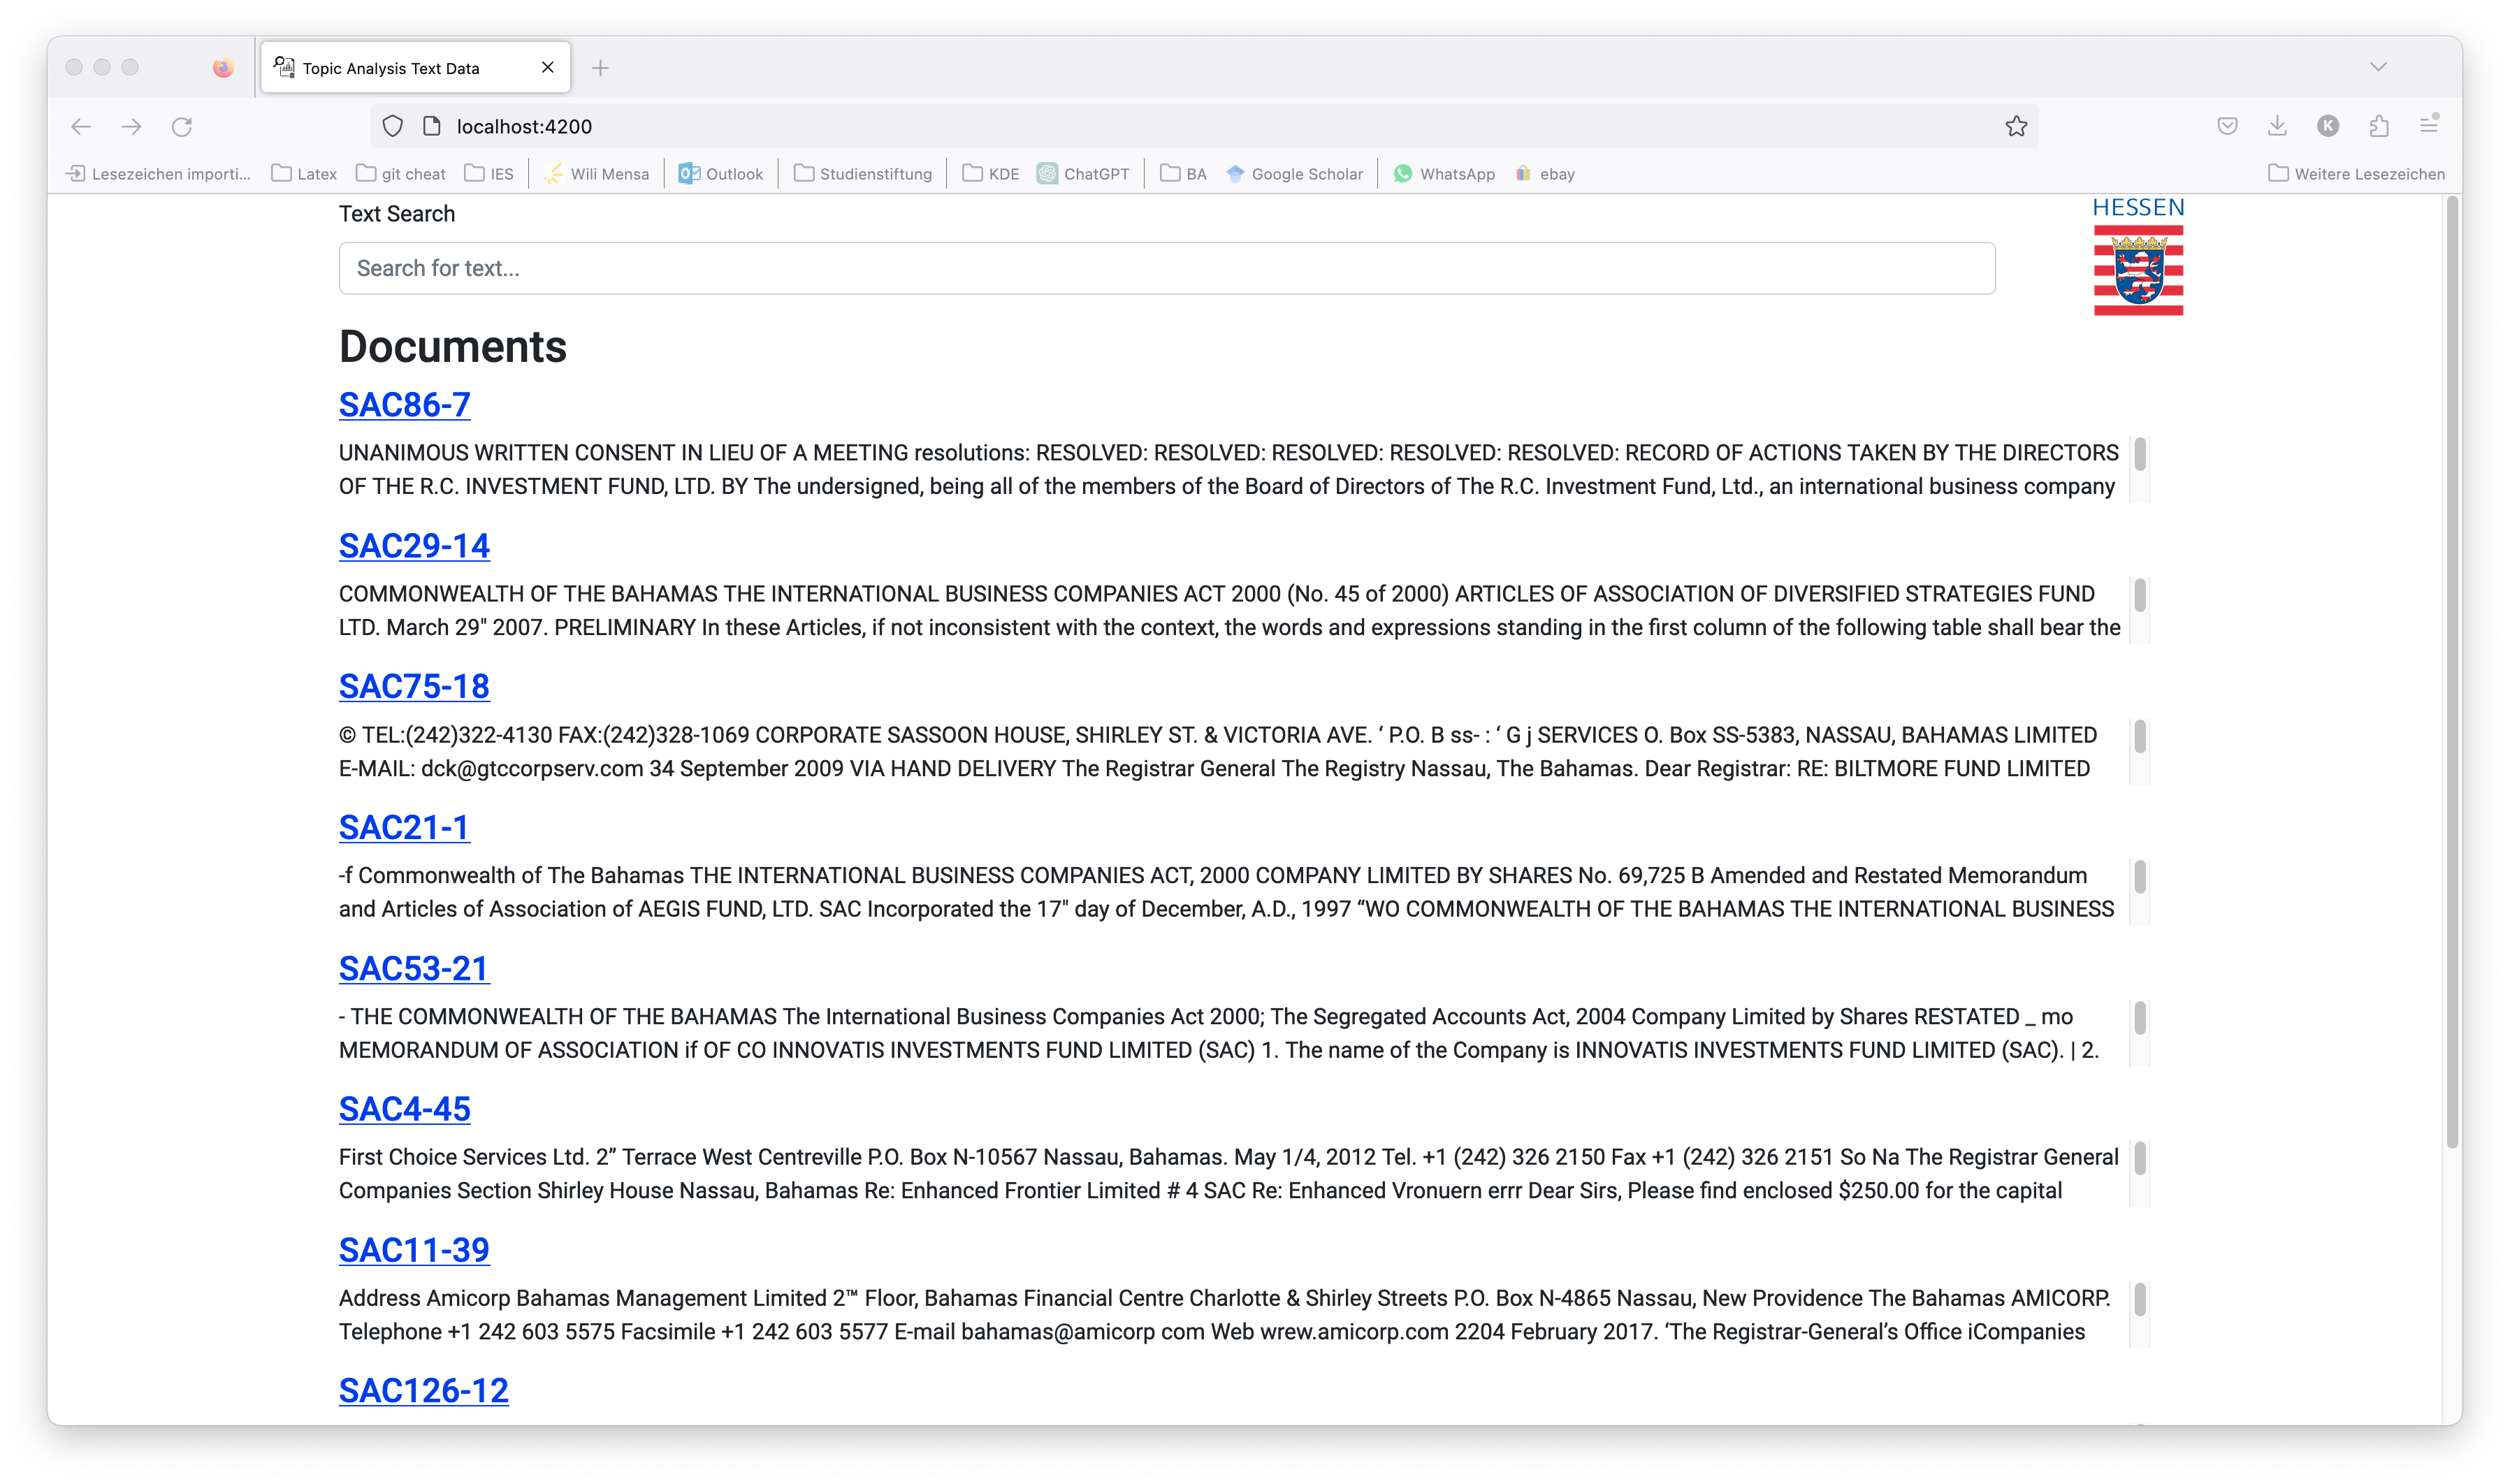
\includegraphics[width=0.7\textwidth]{images/UI/Home_component.png}
    \caption[Home component of the frontend]{Home component of the frontend.
    The search bar is used to enter the text query.
    The results of the query are displayed below the search bar.
    }
    \label{fig:home_comp}
\end{figure}


\begin{figure}[htp] % htp = hier (h), top (t), oder auf einer eigenen Seite (p).
    \centering
    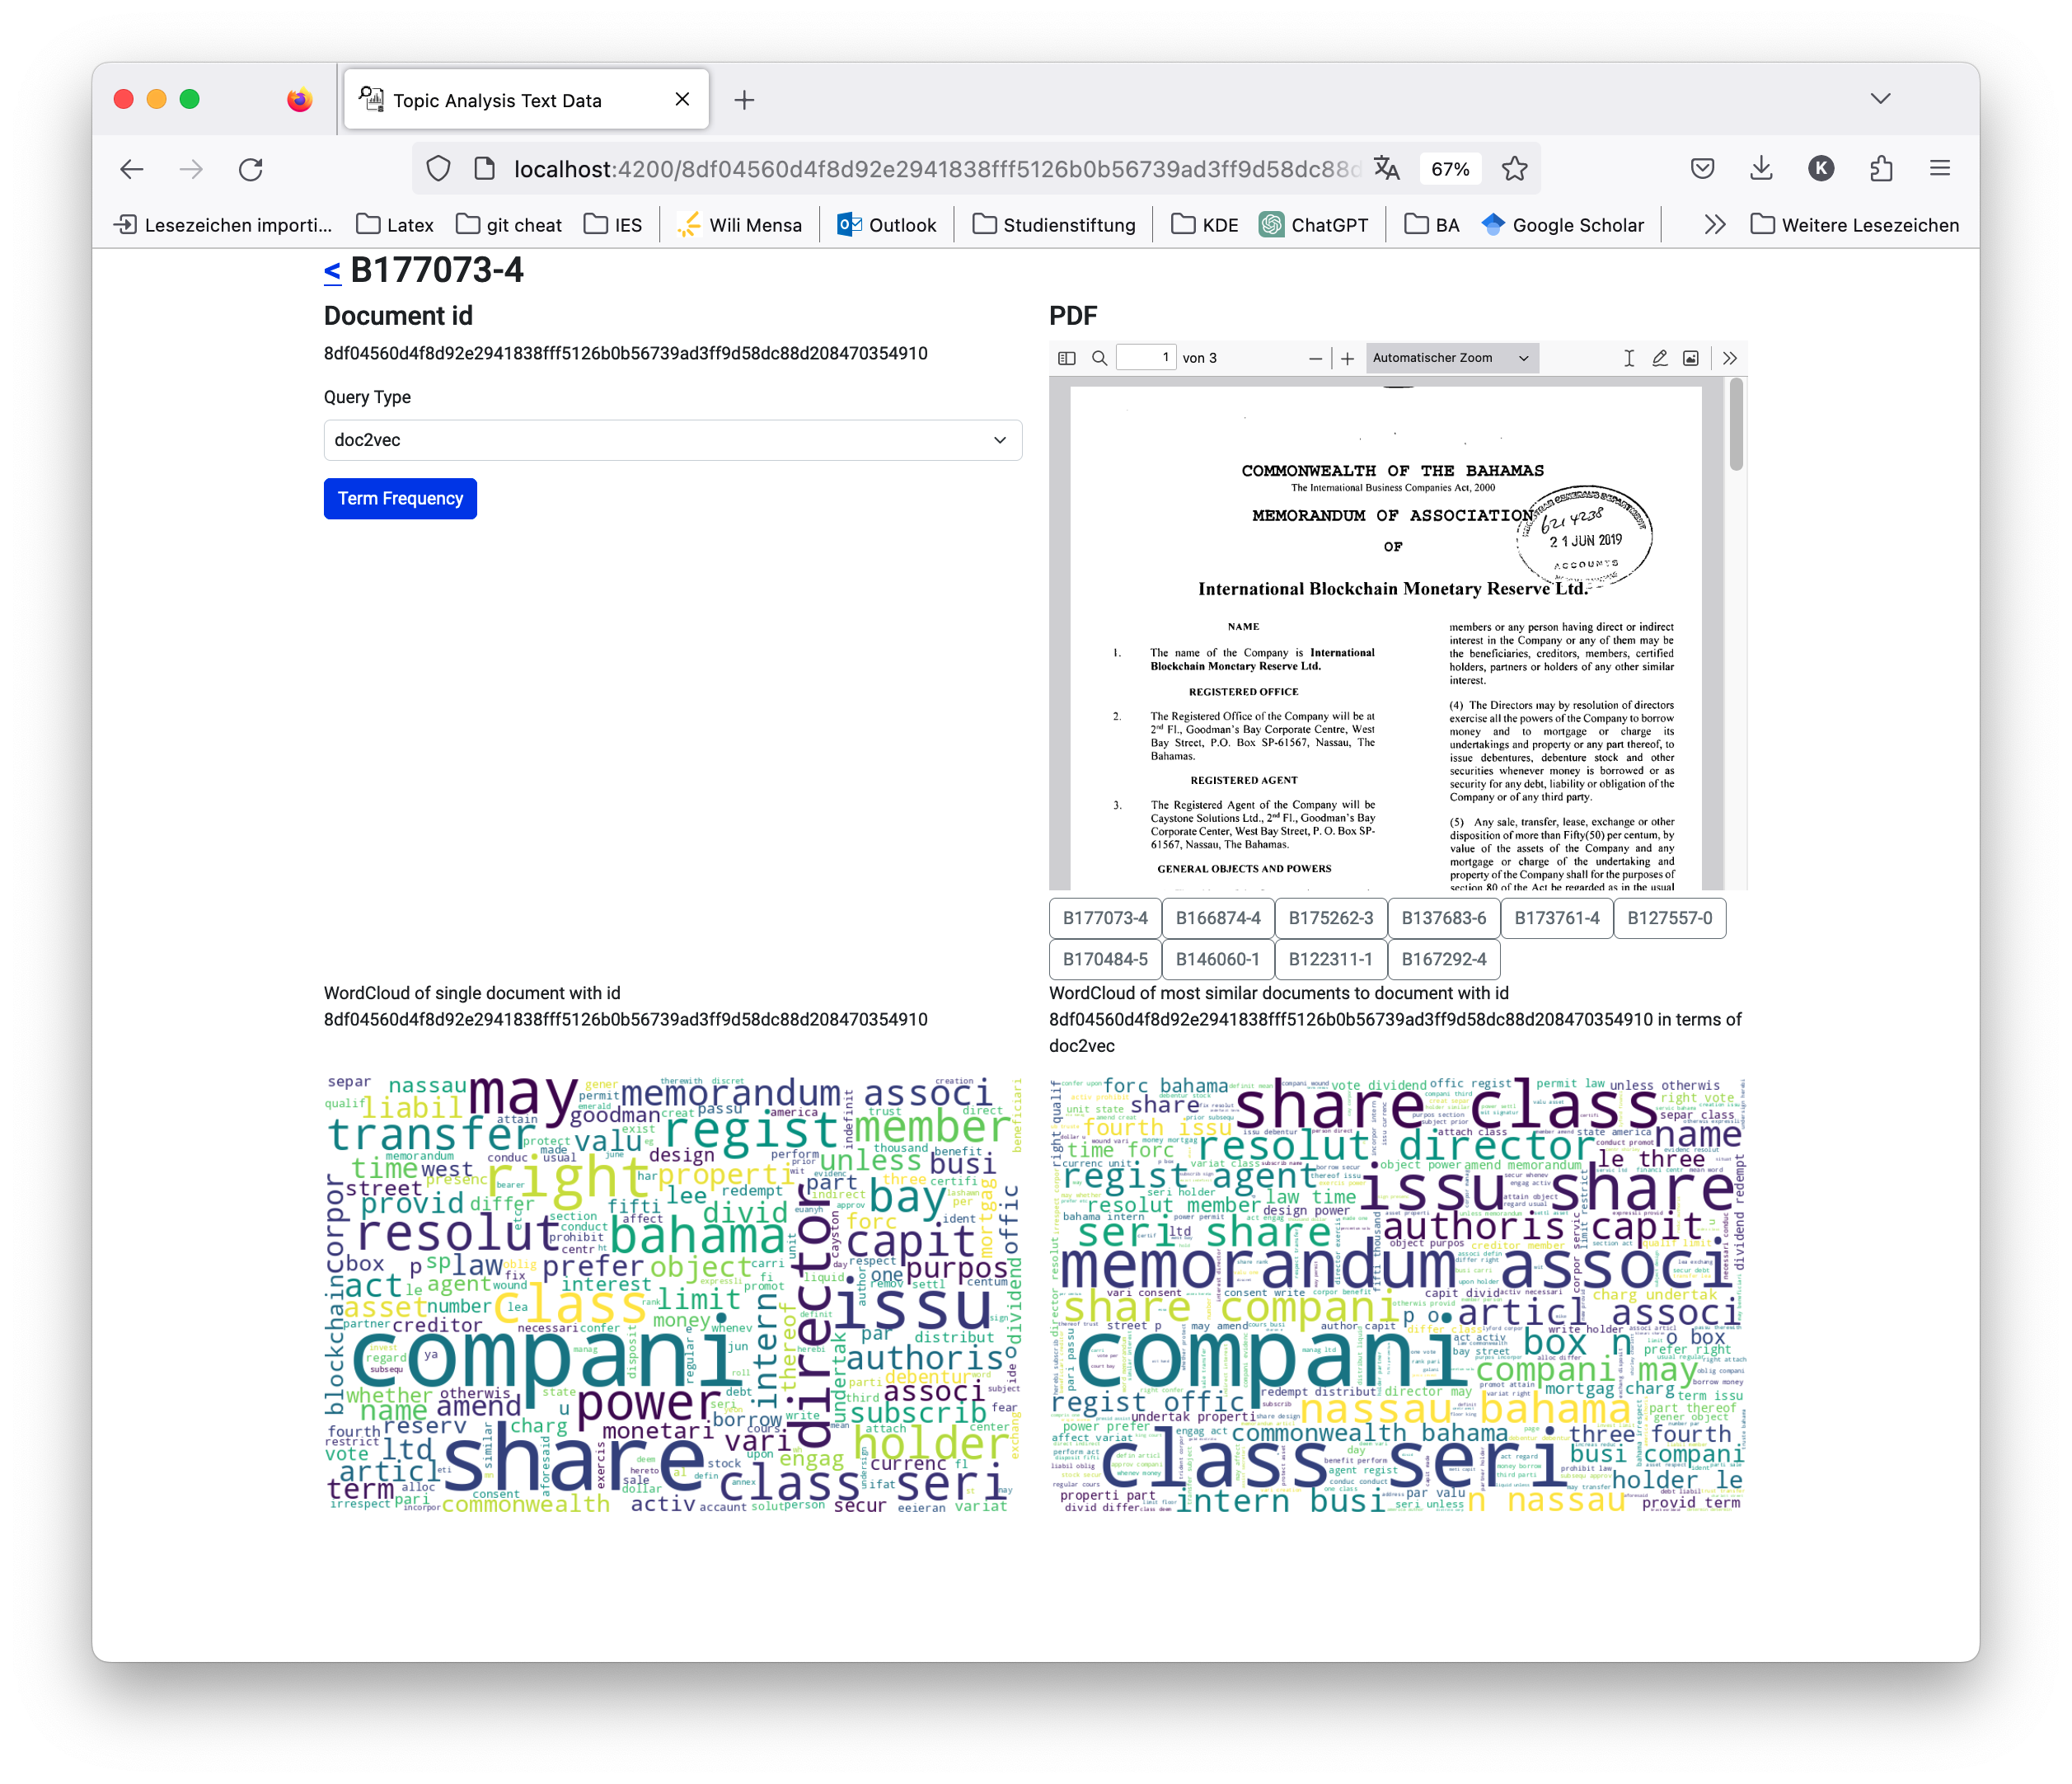
\includegraphics[width=0.7\textwidth]{images/UI/Home_detail.png}
    \caption[Detail component of the frontend]{Detail component of the frontend.
    The chosen document is displayed, as well as its most similar documents in the database.
    WordClouds of the document and the most similar documents are displayed.
    }
    \label{fig:detail_comp}
\end{figure}


\begin{figure}[htp] % htp = hier (h), top (t), oder auf einer eigenen Seite (p).
    \centering
    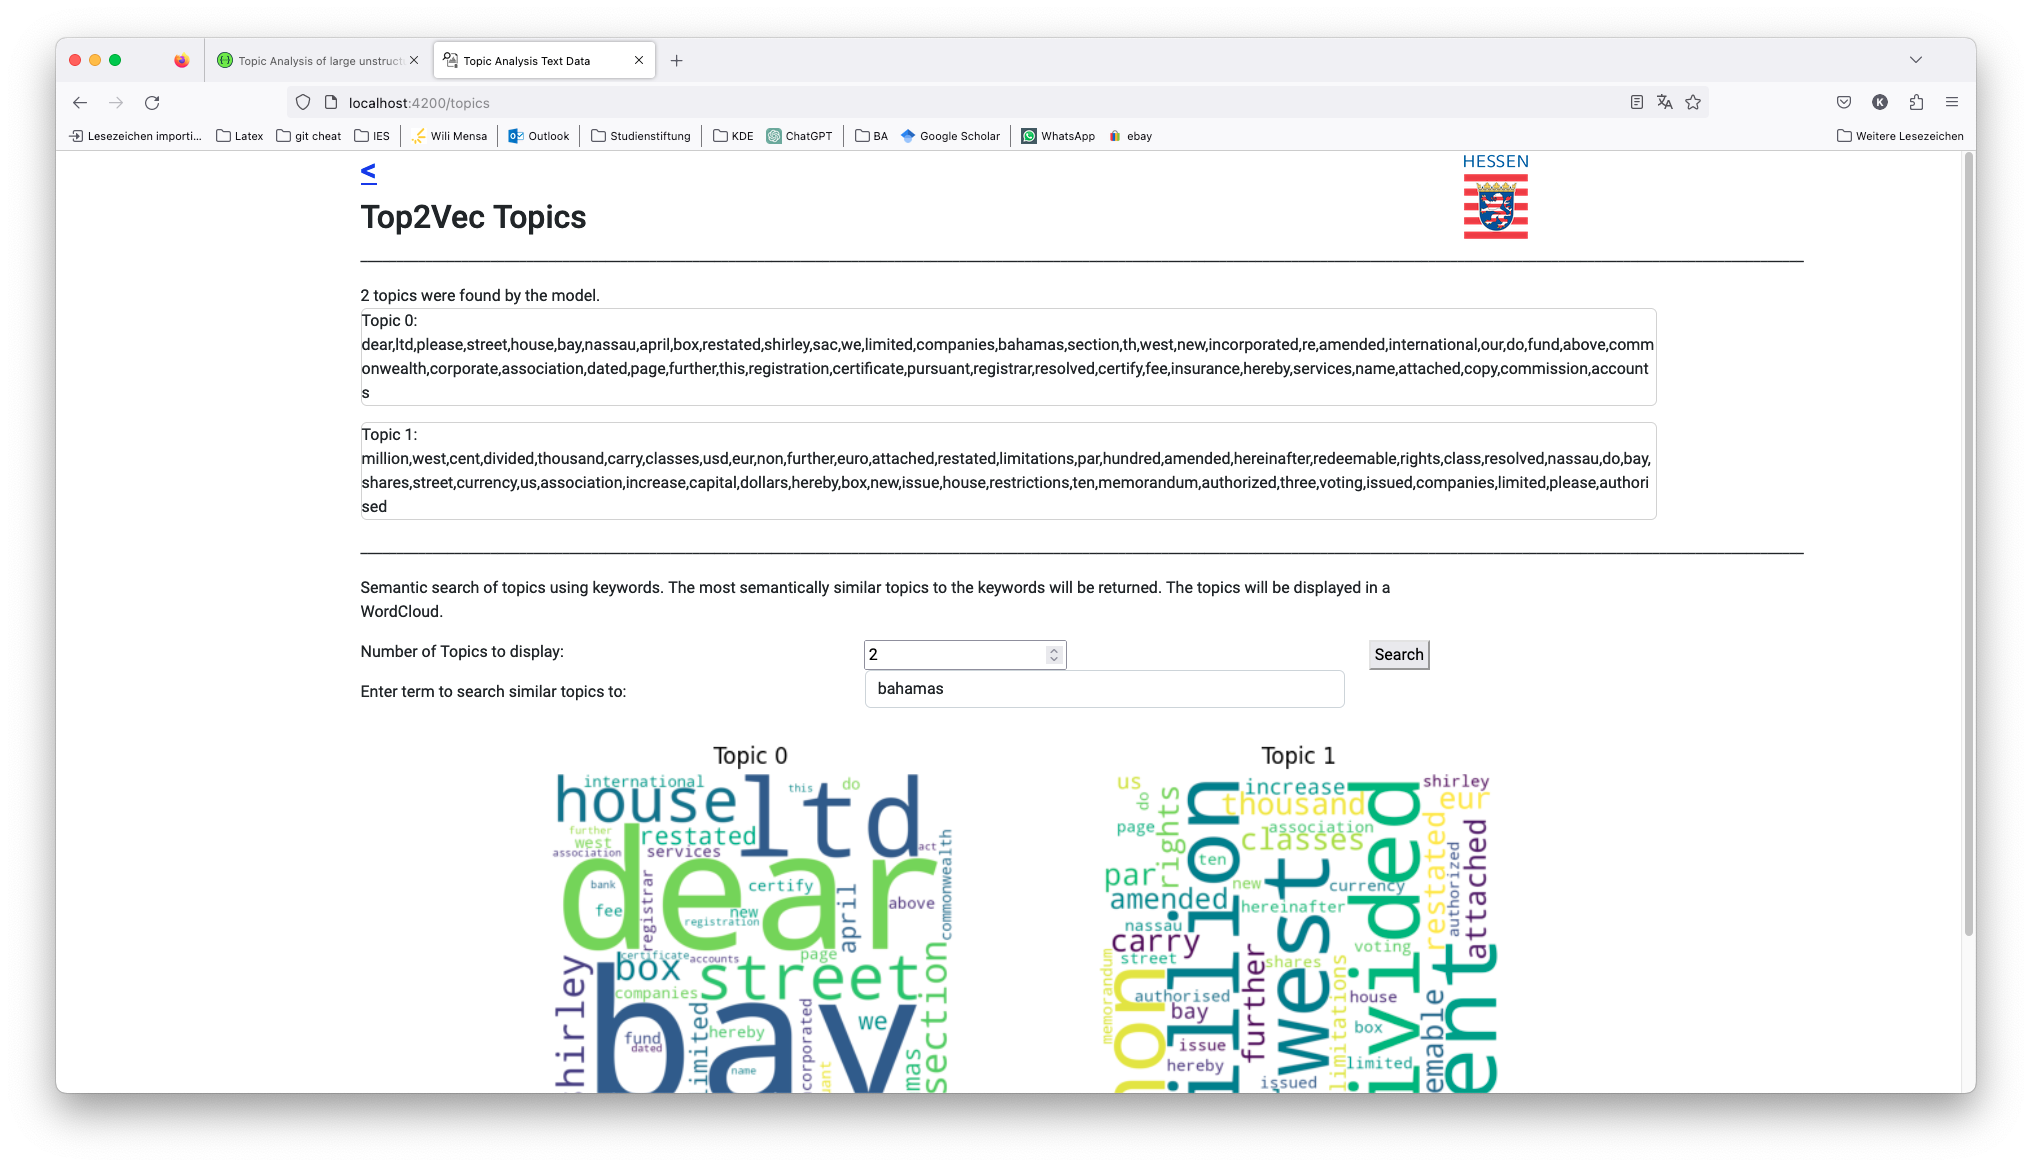
\includegraphics[width=0.7\textwidth]{images/UI/Top2Vec_Topics.png}
    \caption[Topic component of the frontend]{Topic component of the frontend.
    The topics identified by \topTwovec{} are listed.
    Below them, the user can query for the most similar topics to a term.
    The results are displayed as a \wordcloud{}.
    }
    \label{fig:top2vec_topic_comp}
\end{figure}


To change between the components, the routes have to be defined.
The routes are defined in the \texttt{app-routing.module.ts} file, as shown in \autoref{lst:angular_routing}.

\begin{listing}[htp]
    \begin{minted}{typescript}
        const routes: Routes = [
            { path: 'topics', component: TopicsComponent},
            { path: ':id', component: DocumentDetailComponent},
            { path: '', component: HomeComponent},
          ];
    \end{minted}
    \caption{Definition of routes in \angular{} in the \texttt{app-routing.module.ts}.
    }
    \label{lst:angular_routing}
\end{listing}